
The main reason for using keywords is


than for a computer where the content has to be stored in categories


Our overall goal is to make the computer understand the interests of the user by understand texts that the user is interested in, for instance articles read or text on web pages visited. 


the performance by humans could be 

Then human task of content analysis 


i.e., 



The overall goal is to let the computer understand the interests of the user by understanding the content of text. 

The easiest way to perform content analysis for a computer is to find specialized words in texts and find out what these words mean. 

**Some words are more likely to reflect the content of an article than other. 




do categorization of content. 

, and our goal is to make the computer understand different texts. 

. The purpose of understanding the text  




a useful approach for improving user experience or advertising. User experience can be improved by letting the computer know the interests of the user, and therefore make better suggestions. Advertising can be improved by directing the advertisement towards users that are more likely to become customers or consumers. 


On way of achieving content analysis is through contextual classification.  The classification should be an automatic process since there are lots of data to process, and to make the classification possible in all languages with only small changes. 

%Taking use of Wikipedia as a knowledge base would 

%\subsection*{}

%It is almost impossible to find a proper model for large amounts of data if the model is based on training sets, and we will therefore use 
%Problemet: Innnholdsanalyse
%-> brukes i advertising-formål

%kontekstuell  og behavioral reklame -> mer penger for
%mye data -> autmatisk klassifisering. 

%mange teknikker, lager en modell
%utfordinger: umulig a lage treningssett. 
%Teknikk som er lett å bootstrappe, ikke krever noe fra kunden, gir en output som kunden kan forstå, enkelt å variere


%The technique used for 

%lett å bootstrappe og mange språk -> wikipedia er egnet for dette formålet. 


%User experience can be improved by letting the computer know what the interests of the user. There are different ways of achieving %knowledge about the user behavior. One of these approaches is to use contextual classification which is the topic of this article.  

% WHY
%Improving user experienceere
%Advertising. 


%Improving user experience is relevant in many contexts, for instance advertising

% HOw: 


%but this article will discuss the approach of using contextual classification. 



%focus on using contextual classification for 

%User experience can be improved if the computer knows the interests of the user. If the computer for instance understands the content of an article, it could use this to find similar articles within the same topic. One way of finding similarity between documents is by classifying the documents together so that articles of the same topics are linked together.  

%This paper describes the usage of classification of Wikipedia to understand the content, and how this could improve the overall user experience. The article will start with an introduction about Wikipedia and classification in general. The main part of this paper will cover the usage of Wikipedia as a knowledge base for classification, with the purpose of improving the user experience. The paper will discuss some of the applications of the different classification approaches.

%before covering a discussing of the classification applications and a summary of a classification approach.subsection*
I\subsection*{Introduction}

There are a lot of challenges for our classification technique. The result from our classification should be easy to understand for the users of the result, including the non-technical users. This means that the result of our classification should not be measured by some numbers, but should instead be "translated" to a understandable result. 



Finding a good automatic classification has


The paper will start with a short introduction to Classification followed by a short introduction to Wikipedia and why this is a good knowledge base for our classification problem. 


The thought about keywords is that there are some words that are more likely to give away the content of an article. If an article mentions Pippi Langstrømpe (the main character in lots of Astrid Lindgren's children books) is the probability for the article to be about Astrid Lindgren larger than if the articles does not mention the name. 

The main reason for using keywords is


than for a computer where the content has to be stored in categories



to make the computer understand the interests of the user by understand texts that the user is interested in, for instance articles read or text on web pages visited. 
There are a lot of challenges for our classification technique. The result from our classification should be easy to understand for the users of the result, including the non-technical users. This means that the result of our classification should not be measured by some numbers, but should instead be "translated" to a understandable result. 



Finding a good automatic classification has

Classification can be defined as the problem of identifying what category a new observation belongs %\footnote{http://en.wikipedia.org/wiki/Statistical_classification}
i.e., the task of sorting similar elements together by using a function. There are, as already mentioned, different approaches to do classification. \textit{Manual classification} uses experts to decide the class of the input, \textit{rule-base classification} creates rules that decide the class of the input and \textit{statistical classification} uses a training set and 

statics to compute the probabilities of the different class given the input. 




The paper will start with a short introduction to Classification followed by a short introduction to Wikipedia and why this is a good knowledge base for our classification problem. 

In other words, classification is given as the task of sorting elements together given some logic structure. There are three different approaches to achieve classification (see also figure \ref{fig:classification_approaches}): 
\begin{itemize}
\item \textit{Manual classification:} Experts decide the class of the input
\item \textit{Rule-based classification:} Rules decide what classification to achieve
\item \textit{Statistical classification:} Based on some training data set. 
\end{itemize}
The manual classification is the one that usually produce the best result, but is both time consuming and tedious when there are lots of classes and input. The purpose of using machine learning in classification is therefore to automate the repetitive task of deciding the category of some input.

%\begin{figure}
%\centering
%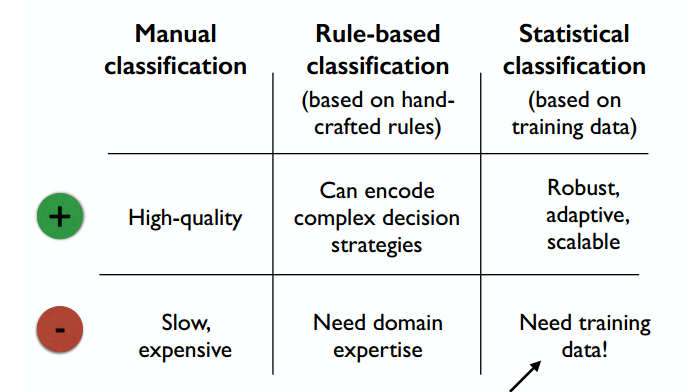
\includegraphics[height=6cm]{classification_approaches}
%\caption{Advantages and disadvantages with different classification approaches}
%\label{fig:classification_approaches}
%\end{figure}
Machine learning is defined as the technique of teaching the machine how to behave, where our result usually is a process where we learn the machine how to behave given some input. The process is about finding patterns or to predict, and the goal for the process is that the behavior becomes as optimal as possible. 
There are three approaches of learning within machine learning: supervised learning, reinforcement learning and unsupervised learning. 
\begin{itemize}
\item \textit{Supervised learning} is a technique where the machine is given a training data set. The training data set in supervised learning is a data set that contains the correct output in addition to the input we want to classify. The classifier can use this data to train the classifier so it returns the wanted output.
\item \textit{Reinforcement learning} is a machine learning approach where the machine receives some feedback about the result of the actions made.   This can either be after each action, or at the end. 
\item \textit{Unsupervised learning} is the task of trying to find a hidden structure in labeled data. The difference is that the classifier receives no feedback about the result. 
\end{itemize}
There are of course advantages and disadvantages with all approaches listed above, and which method to choose is decided by the problem definition.

In this classification problem is a unsupervised classification preferable. Trying to solve the problem with supervised classification would lead to some problems; it is almost impossible to create a training set for such a large data set that we could base our model on and it is difficult to adjust the model to fit changes. 

%Classification as a part of machine learning, is the process where we give some input to the machine (at set of objects) and want to get outputs (the categories) in which they belong. The process is to find the function, also called classifier, that predicts the output for any input. This is usually written as

%\[\gamma: X \rightarrow Y \]

%Classification is  usually either supervised, where we give a training set with the correct output, or it is unsupervised, where the classifier tries to find common features in the data and categorize based on this. 

@article{Breaklines,
author = {Donald E. Knuth and Michael F. Plass},
title = {Breaking Paragraphs into Lines},
journal = {Software---Practice and Experience},
volume = 11,
year = 1981,
pages = {1119-1184}
}

@ONLINE{Entityextraction,
    author = {Abhishek Gattani, Digvijay S. Lamba, Nikesh Garera, Mitul Tiwari, Xiaoyong Chai, Sanjib Das,  Sri Subramaniam,  Anand Rajaraman, Venky Harinarayan, AnHai Doan},
    organization = {},
    url = {http://pages.cs.wisc.edu/~anhai/papers/doctagger-vldb13.pdf},
    title = {Entity Extraction, Linking, Classification, and Tagging for Social Media: A Wikipedia-Based Approach},
    month = aug,
    year = {2013},
}

@ONLINE{Example,
    author = {Abhishek Gattani, Digvijay S. Lamba, Nikesh Garera, Mitul Tiwari, Xiaoyong Chai, Sanjib Das,  Sri Subramaniam,  Anand Rajaraman, Venky Harinarayan, AnHai Doan},
    organization = {Google Machine Translation Team},
    url = {http://pages.cs.wisc.edu/~anhai/papers/doctagger-vldb13.pdf},
    title = {All Our N-Gram are Belong to You},
    month = aug,
    year = {2006},
}

@ONLINE{Nowikidump, 
    author = {},
    url = {http://dumps.wikimedia.org/nowiki/latest/},
    organization = {},
    title={},
    month = aug,
    year = {},
}

@ONLINE{Categorytree, 
    author = {},
    url = {http://no.wikipedia.org/w/index.php?title=Spesial%3AKategoritre&target=Astrid+Lindgren&mode=categories&namespaces=},
    organization = {},
    title={},
    month = aug,
    year = {},
}

@ONLINE{Olejohandahleng, 
    author = {},
    url = {http://en.wikipedia.org/wiki/Ole-Johan_Dahl},
    organization = {},
    title={},
    month = aug,
    year = {},
}

@ONLINE{IABabout, 
    author = {},
    url = {http://www.iab.net/about_the_iab},
    organization = {},
    title={},
    month = aug,
    year = {},
}

@ONLINE{Encknowledge,
    author = {Abhishek Gattani, Digvijay S. Lamba, Nikesh Garera, Mitul Tiwari, Xiaoyong Chai, Sanjib Das,  Sri Subramaniam,  Anand Rajaraman, Venky Harinarayan, AnHai Doan},
    organization = {Google Machine Translation Team},
    url = {{http://pdf.aminer.org/000/012/837/overcoming_the_brittleness_bottleneck_using_wikipedia_enhancing_text_categorization_with.pdf},
    title = {All Our N-Gram are Belong to You},
    month = october,
    year = {2014},
    note = {Accessed: 10-10-2014},
}


%\documentclass[english,a4paper]{ifimaster}
%\usepackage[utf8]{inputenc}
%\usepackage[T1]{fontenc,url}
%\urlstyle{sf}
%\usepackage{babel,textcomp,csquotes,ifimasterforside,varioref,graphicx}
%\usepackage[backend=bibtex,style=numeric-comp]{biblatex}
%\usepackage{wrapfig}
%\usepackage{subcaption}
%\usepackage{float}
%\usepackage{fancyvrb}

%\documentclass[]{uiophd}